%%%%%%%%%%%%%%%%%%%%%%%%%%%%%%%%%%%%%%%%%
% Memo
% LaTeX Template
% Version 1.0 (30/12/13)
%
% This template has been downloaded from:
% http://www.LaTeXTemplates.com
%
% Original author:
% Rob Oakes (http://www.oak-tree.us) with modifications by:
% Vel (vel@latextemplates.com)
%
% License:
% CC BY-NC-SA 3.0 (http://creativecommons.org/licenses/by-nc-sa/3.0/)
%
%%%%%%%%%%%%%%%%%%%%%%%%%%%%%%%%%%%%%%%%%

\documentclass[letterpaper,11pt]{texMemo} % Set the paper size (letterpaper, a4paper, etc) and font size (10pt, 11pt or 12pt)

\usepackage{parskip} % Adds spacing between paragraphs
\setlength{\parindent}{15pt} % Indent paragraphs

%----------------------------------------------------------------------------------------
%	MEMO INFORMATION
%----------------------------------------------------------------------------------------

\memoto{Dr. Max Donath} % Recipient(s)

\memofrom{Mr. Dingyi Gu} % Sender(s)

\memosubject{ME 5286 Robotics Lab1} % Memo subject

\memodate{Tuesday, February 11, 2020} % Date, set to \today for automatically printing todays date
 
\logo{\includegraphics[width=0.3\textwidth]{logo.eps}} % Institution logo at the top right of the memo, comment out this line for no logo

%----------------------------------------------------------------------------------------



\renewcommand{\thesubsection}{\arabic{subsection}}
\makeatletter
\def\@seccntformat#1{\@ifundefined{#1@cntformat}%
	{\csname the#1\endcsname\quad}%    default
	{\csname #1@cntformat\endcsname}}% enable individual control
\newcommand\section@cntformat{}     % section level 
\makeatother


\usepackage{graphicx} %This one allows you to import images.
\usepackage{float} %Allows for control of float positions


%subfig
\usepackage{caption}

\usepackage{subfig}
\usepackage{setspace}


\begin{document}

\maketitle % Print the memo header information

%----------------------------------------------------------------------------------------
%	MEMO CONTENT
%----------------------------------------------------------------------------------------


\doublespacing

\section{Task1-3}

\subsection{Describe the difference between joint and Cartesian space and how that affected the	motion of the robot.}

Cartesian space is defined by the position and orientation of the end effector of a robot, which is broken down into X, Y and Z coordinates in a simple grid. While joint space is defined by a vector whose components are the translational and angular displacements of each joint of a robotic link. When applying Cartesian space along the kinematic chain, often you will analyze the position of one link with respect to the next link as a new coordinate system. However, this kind of information is not always particularly helpful in robotics. Depending on where it is, there might be a number of ways to position its end effector in a certain location, and it could be hard to tell a robotic arm to reach there. So instead, you tell each of its joints exactly what position to be in. By giving robot the angles each joint should be, the robot can then move to the desired location. 

\subsection{Describe the limitations of the robot’s workspace based upon the mounting location of the robot on the table.}

When you add a target which is quite close to the workspace, the UR5 robot may touch the table because of different configurations (like the arm is elbow down) in both RoboDK simulation and real situation, where the robot should stop its motion. As a result, it is really important for us to check and modify the configuration once the target is added. Otherwise the robot will generate configuration in relation to the embedded algorithm, which contains the collision between the robot and the table. It is essential to double check it before implementing the program linked to the selected robot.

\subsection{Show the usable workspace of the robot. Use a program (Matlab, Excel, etc.) to plot the workspaces. This can either be a 3D view or multiple 2D views.}

%\begin{figure}[H]
%	\centering
%	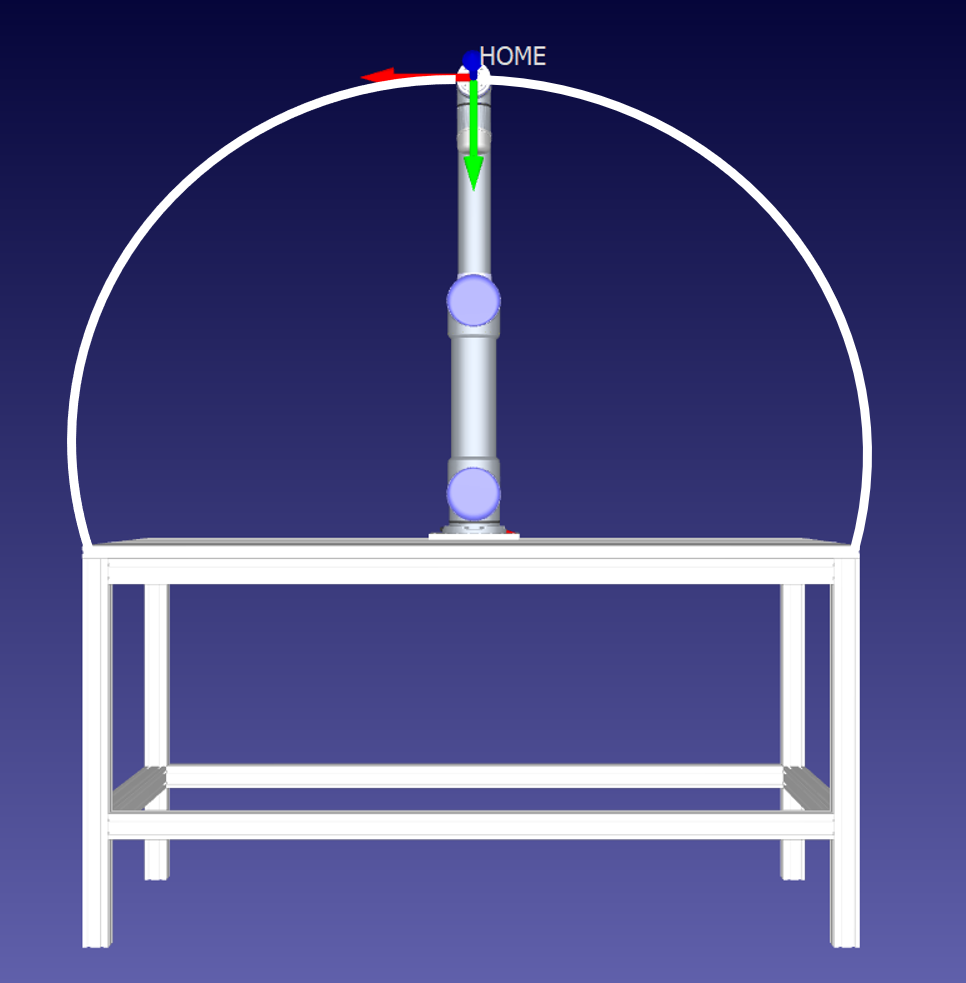
\includegraphics[height=1.4in]{C:/Document_Dingyi/UMN/Spring_2020/ME5286/Lab1/Lab_memo/figures/Left.png}
%	\caption{System Block Diagram}
%	\label{fig:1}
%\end{figure} 	

%C:/Document_Dingyi/UMN/Spring_2020/ME5286/Lab1/Lab_memo/figures/Left.png

\begin{figure}[H]
	\centering   
	\subfloat[Front view]{
		\label{fig:1:a} %% label for first subfigure
		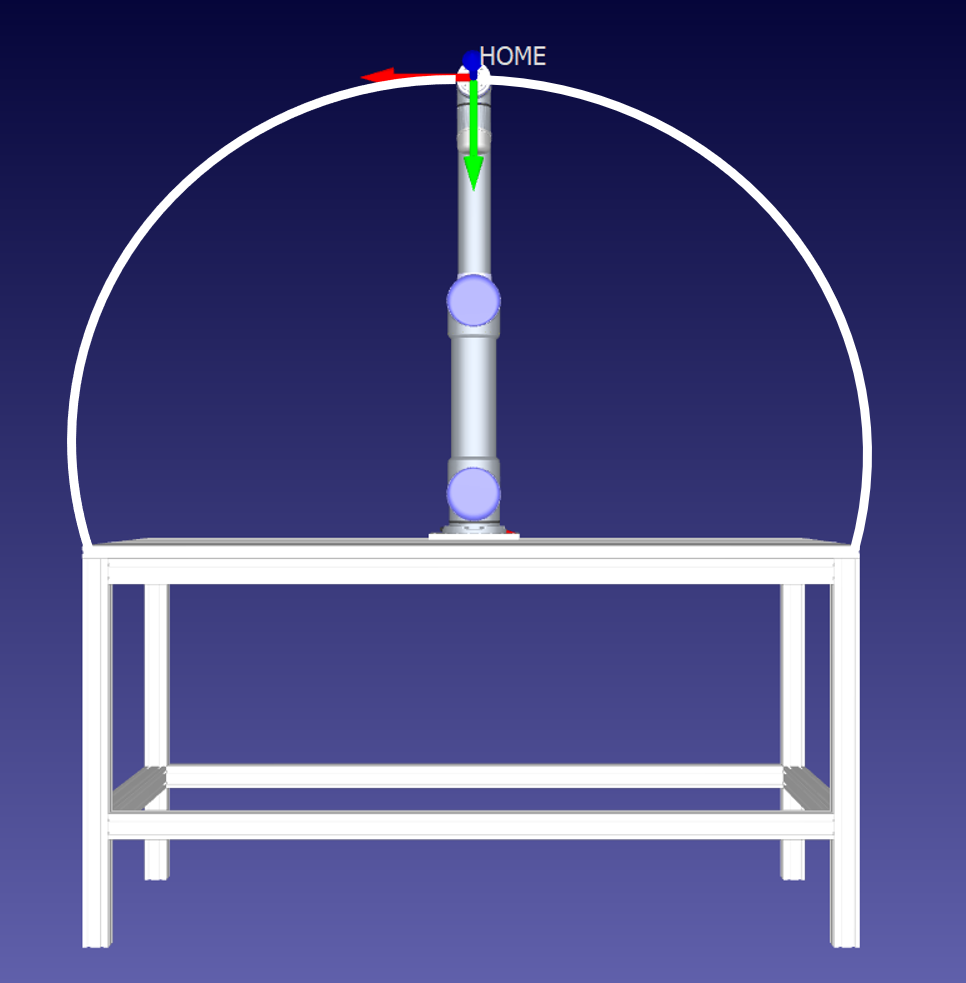
\includegraphics[height=2in]{C:/Document_Dingyi/UMN/Spring_2020/ME5286/Lab1/Lab_memo/figures/Left.png}}
	\hspace{0.1in} 
	\subfloat[Side view]{
		\label{fig:1:b} %% label for second subfigure
		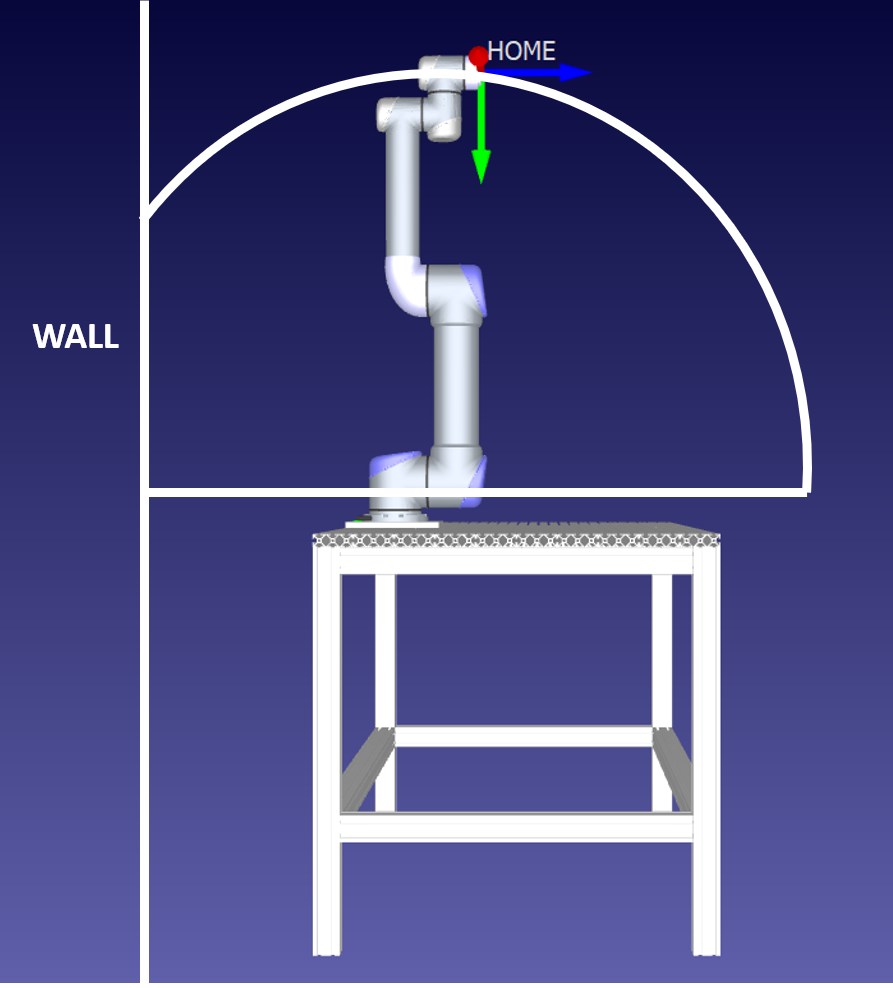
\includegraphics[height=2in]{C:/Document_Dingyi/UMN/Spring_2020/ME5286/Lab1/Lab_memo/figures/Back.png}}
	\hspace{0.1in}
	\subfloat[Top view]{
		\label{fig:1:c} %% label for second subfigure
		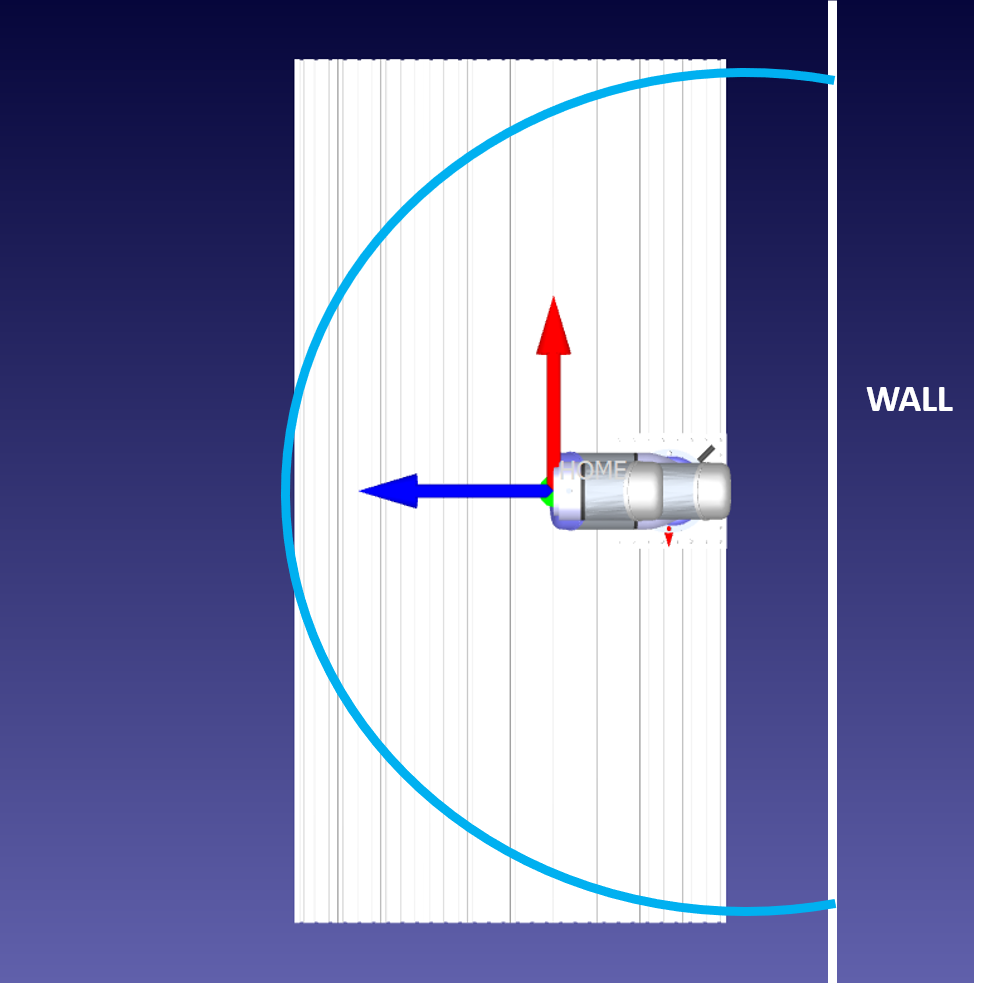
\includegraphics[height=2in]{C:/Document_Dingyi/UMN/Spring_2020/ME5286/Lab1/Lab_memo/figures/Top.png}}
	\caption{Usable workspace of the robot UR5 } 
	\label{fig:1}
\end{figure}

Fig.~\ref{fig:1} presents the edges of the usable workspace, and the robot cannot go under the table and behind the wall as well.


\subsection{What are the two safety planes? And how did you determine where they were?}

The first one is offset from the table surface corresponding to the usable workspace in qn3. The second one is behind the robot and parallel to the wall.



\subsection{Is the robot elbow up or elbow down for these tasks? How do you know and how did you ensure that the robot chose this elbow configuration?}

Initially at some targets, the robot was elbow down. We modified the elbow by clicking configuration at different waypoints in order to make sure there is no collision between the elbow and the table.


\subsection{Define what “collaborative” means when talking about “collaborative robotics”? What makes the robot collaborative?}

Collaborative robot is the robot that is able to work or interact with human in a shared workspace. “Collaborate” means there are some features for cobot: safety monitored stop, hand guiding, speed and separation monitoring, power and force limiting. Therefore, “collaborative” defines that the cobot should be designed by working
together with human. Cobot is able to monitor the space between itself and human and stop moving when it might cause danger to people. For example, when people step into pre-designed safety zone, the robot will slow down the speed or stop when getting too
close. The power and force limiting feature of robot can detect the overload force on itself and slow down or stop when needed. Therefore, people can safely work with cobot without any additional safety devices.

\subsection{Compare and contrast the three programming methods. Which do you find easiest to use at the moment? Which method seems to have the most capabilities or lack of capabilities? Which method do you foresee yourself using for the rest of the class?}

The easiest one to use at the moment is RoboDK. RoboDK Python API has the most capability. PolyScope has lack of capability because every step and motion of robot need to be manually controlled by myself using the tablet. I preferred to work with RoboDK Python API for the rest of the class.


\section{Task4}

\subsection{Create a table showing the vertices you used in the cube and describe how you picked	these vertices}


\renewcommand\arraystretch{2}
\begin{table}[H]\footnotesize
\centering
\begin{tabular}{|c|c|c|c|c|c|c|}
\hline
 & \textbf{X($mm$)}&\textbf{Y($mm$)}&\textbf{Z($mm$)}& \textbf{RotX($deg$)} & \textbf{RotY($deg$)} & \textbf{RotZ($deg$)} \\
\hline
Home & 0.000 & -191.000 & 1000.280 & 90.000 & 0.000 & 180.000\\
\hline
Target1 & -300.000 & -600.000 & 600.000 & 90.000 & 0.000 & 180.000\\
\hline
Target2 & -200.000 & -600.000 & 600.000 & 90.000 & 0.000 & 180.000\\
\hline
Target3 & -200.000 & -600.000 & 520.000 & 90.000 & 0.000 & 180.000\\
\hline 
Target4 & -300.000 & -600.000 & 520.000 & 90.000 & 0.000 & 180.000\\
\hline
Target5  & -300.000 & -100.000 & 520.000 & 90.000 & 0.000 & 180.000\\
\hline
Target6  & -300.000 & -100.000 & 600.000 & 90.000 & 0.000 & 180.000\\
\hline
Target7  & -200.000 & -100.000 & 600.000 & 90.000 & 0.000 & 180.000\\
\hline
Target8  &-200.000 & -100.000 & 520.000 & 90.000 & 0.000 & 180.000\\
\hline
\end{tabular}
\caption{Vertices picked for maximum length in y-direction}
\label{table:1}
\end{table}

Table.~\ref{table:1} shows the vertices I picked for the maximum length in y-direction. To begin with, the robot started from the home position to Target1. In order to form the complete prism motion in 100$mm$ $\times$ 500$mm$ $\times$ 80$mm$, the robot moved from 1-2-3-4-5-6-7-8-3-2-7-6-1. Fig.~\ref{fig:2:a} shows the trajectory in y-direction.

%\begin{figure}[H]
%	\centering
%	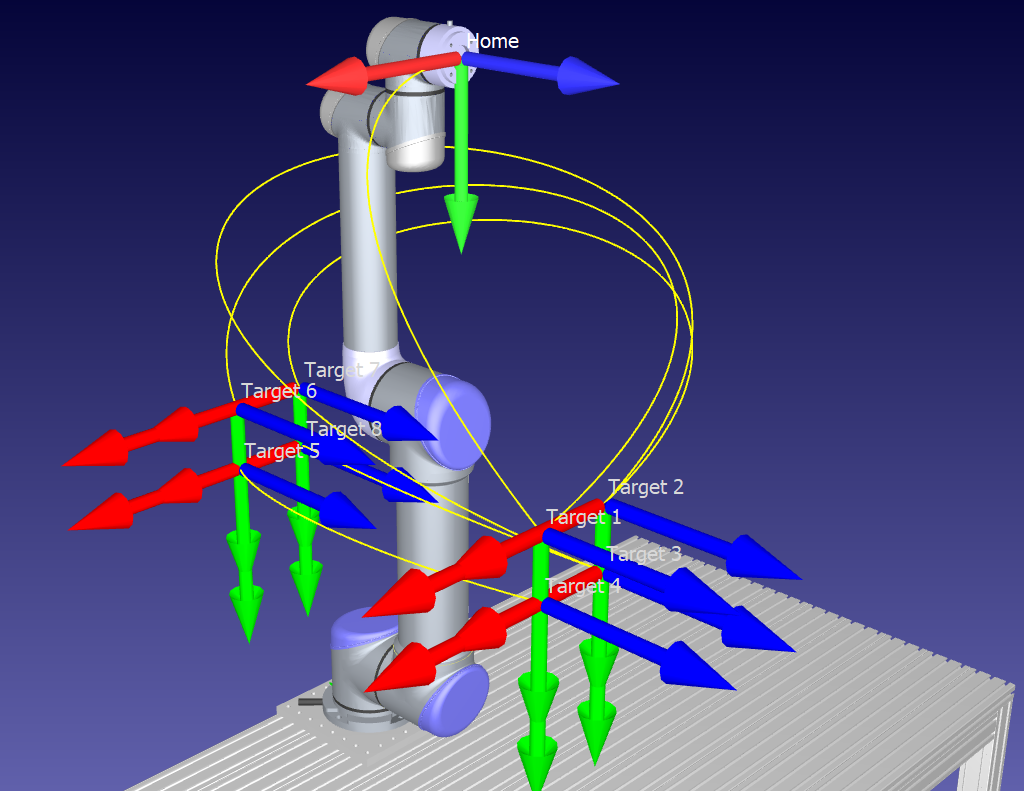
\includegraphics[height=2.4in]{C:/Document_Dingyi/UMN/Spring_2020/ME5286/Lab1/Lab_memo/figures/task4y.png}
%	\caption{Taks4 in y-direction}
%	\label{fig:2}
%\end{figure} 	

\begin{figure}[H]
	\centering   
	\subfloat[Front view]{
		\label{fig:2:a} %% label for first subfigure
		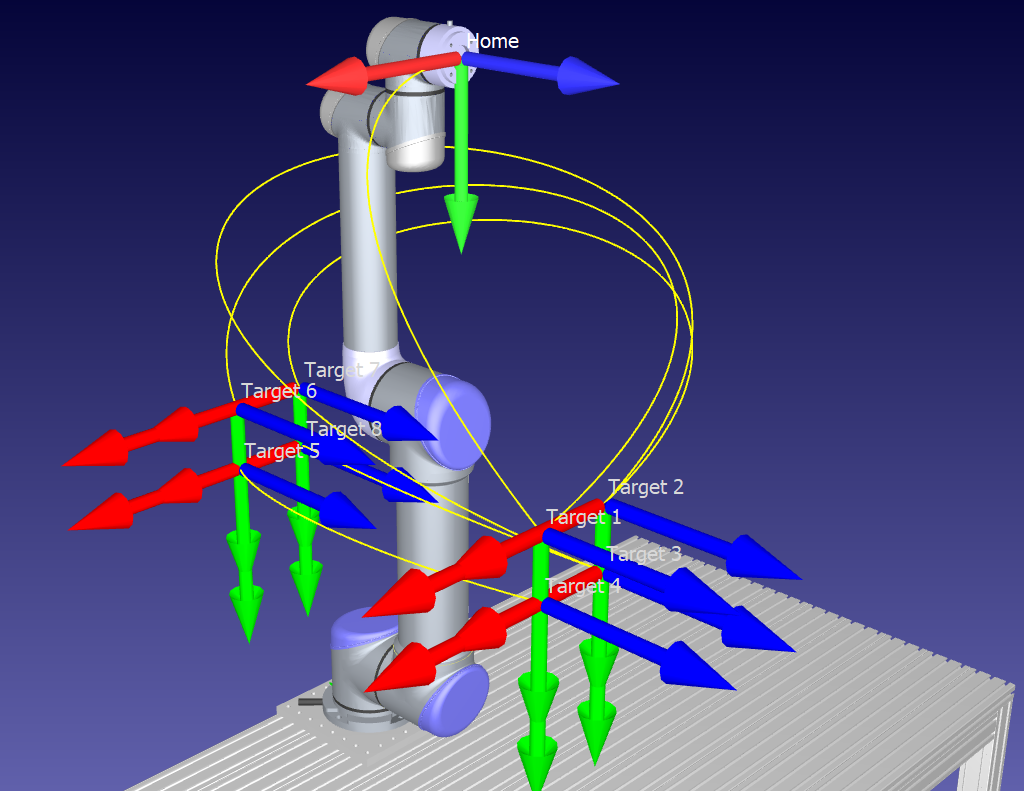
\includegraphics[height=2.2in]{C:/Document_Dingyi/UMN/Spring_2020/ME5286/Lab1/Lab_memo/figures/task4y.png}}
	\hspace{0.1in} 
	\subfloat[Side view]{
		\label{fig:2:b} %% label for second subfigure
		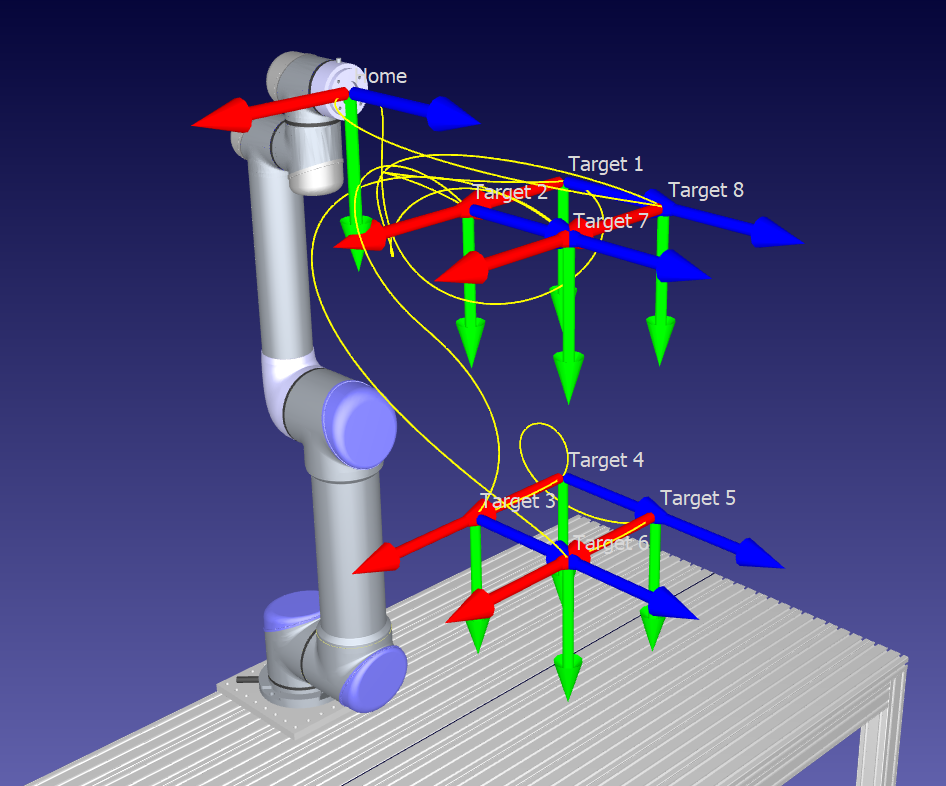
\includegraphics[height=2.2in]{C:/Document_Dingyi/UMN/Spring_2020/ME5286/Lab1/Lab_memo/figures/task4z.png}}
	\caption{Task 4 } 
	\label{fig:2}
\end{figure}


\renewcommand\arraystretch{2}
\begin{table}[H]\footnotesize
	\centering
	\begin{tabular}{|c|c|c|c|c|c|c|}
		\hline
		& \textbf{X($mm$)}&\textbf{Y($mm$)}&\textbf{Z($mm$)}& \textbf{RotX($deg$)} & \textbf{RotY($deg$)} & \textbf{RotZ($deg$)} \\
		\hline
		Target1 & 400.000 & -200.000 & 800.000 & 90.000 & 0.000 & 180.000\\
		\hline
		Target2 & 200.000 & -200.000 & 800.000 & 90.000 & 0.000 & 180.000\\
		\hline
		Target3 & 200.000 & -200.000 & 300.000 & 90.000 & 0.000 & 180.000\\
		\hline 
		Target4 & 400.000 & -200.000 & 300.000 & 90.000 & 0.000 & 180.000\\
		\hline
		Target5  & 400.000 & -400.000 & 300.000 & 90.000 & 0.000 & 180.000\\
		\hline
		Target6  & 200.000 & -400.000 & 300.000 & 90.000 & 0.000 & 180.000\\
		\hline
		Target7  & 200.000 & -400.000 & 800.000 & 90.000 & 0.000 & 180.000\\
		\hline
		Target8  &-400.000 & -400.000 & 800.000 & 90.000 & 0.000 & 180.000\\
		\hline
	\end{tabular}
	\caption{Vertices picked for maximum length in z-direction}
	\label{table:2}
\end{table}


Table.~\ref{table:2} shows the vertices picked by my partner Steven. The trajectory was presented in Fig.~\ref{fig:2:b}



\subsection{What does that tell you about the robot’s workspace?}

When picking the vertices of prism, some targets might be not reachable for the robot arm. We need make sure these targets are not too far from or too close to the home position. In addition, you cannot stretch too much on z or
y direction because the target might go under the table or behind the wall. Run the simulation before starting on the real robot to fix errors. 


\subsection{Include a screenshot or figure of the robot trajectory tracing the two cubes.}

Please see details in Fig.~\ref{fig:2}.

\cleardoublepage

\section{Task5}

\subsection{Create a graph showing the force exerted by the robot vs. speed of the robot. (To do this, average the three forces measured at each speed and plot this average force vs speed)}

\begin{figure}[H]
	\centering
	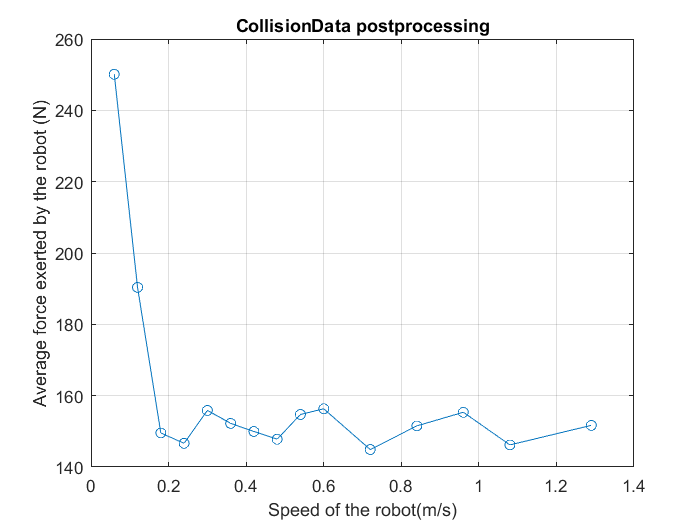
\includegraphics[height=2.5in]{C:/Document_Dingyi/UMN/Spring_2020/ME5286/Lab1/Lab_memo/figures/task5.png}
	\caption{Taks5}
	\label{fig:3}
\end{figure} 	

Fig.~\ref{fig:3} presents the relationship between average force and speed during the collision experiment.



\subsection{What does this graph say about the UR5 strategy for preventing excessive forces when colliding?}

According to Fig.~\ref{fig:3}, when the speed increases, there is a huge drop for force exerted on the robot from (0,0.2$m/s$) , which means the colliding force decreases significantly in order to prevent from excessive damage. This phenomenon help cancel the effect made by speed which is larger than 0.2$m/s$ and protect the robot itself.


\subsection{What was the maximum force recorded and at which speed?}

The maximum force was recorded as 250.12$N$ at 0.06 $m/s$.




%----------------------------------------------------------------------------------------

\end{document}